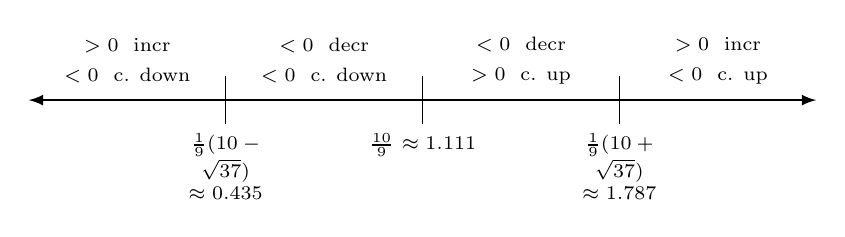
\begin{tikzpicture}[>=latex]

\draw [<->, thick] (-5,0) -- (5,0);
\foreach \x / \y  in %
					{-2.5/{$\frac19(10-\sqrt{37})$ $\approx 0.435$},%
					0/{$\frac{10}9$  $\approx 1.111$},%
					2.5/{$\frac19(10+\sqrt{37})$ $\approx 1.787$}}
		{\draw (\x,-.3) node[below] {\scriptsize \parbox{40pt}{\centering \y}} -- (\x,.3);}
		
\draw (-3.75,.5) node {\scriptsize \parbox{50pt}{\centering $\fp>0$ \ incr \vskip 3pt $\fpp<0$ \ c. down}};
\draw (-1.25,.5) node {\scriptsize \parbox{50pt}{\centering $\fp<0$ \ decr \vskip 3pt$\fpp<0$ \ c. down}};
\draw (1.25,.5) node {\scriptsize \parbox{50pt}{\centering $\fp<0$ \ decr \vskip 3pt $\fpp>0$ \ c. up}};
\draw (3.75,.5) node {\scriptsize \parbox{50pt}{\centering $\fp>0$ \ incr \vskip 3pt $\fpp<0$ \ c. up}};


\end{tikzpicture}